\documentclass[10pt,twocolumn,letterpaper]{article}

\usepackage{iccv}
\usepackage{times}
\usepackage{epsfig}
\usepackage{graphicx}
\usepackage{amsmath}
\usepackage{amssymb}

\usepackage{algorithm}% http://ctan.org/pkg/algorithm
\PassOptionsToPackage{noend}{algpseudocode}% comment out if want end's to show
\usepackage{algpseudocode}% http://ctan.org/pkg/algorithmicx

\makeatletter
\newcommand*{\skipnumber}[2][1]{%
   {\renewcommand*{\alglinenumber}[1]{}\State #2}%
   \addtocounter{ALG@line}{-#1}}
\makeatother

% \newcommand*{\algrule}[1][\algorithmicindent]{\makebox[#1][l]{\hspace*{.5em}\vrule height .75\baselineskip depth .25\baselineskip}}%

% \newcount\ALG@printindent@tempcnta
% \def\ALG@printindent{%
%     \ifnum \theALG@nested>0% is there anything to print
%         \ifx\ALG@text\ALG@x@notext% is this an end group without any text?
%             % do nothing
%             \addvspace{-3pt}% FUDGE for cases where no text is shown, to make the rules line up
%         \else
%             \unskip
%             % draw a rule for each indent level
%             \ALG@printindent@tempcnta=1
%             \loop
%                 \algrule[\csname ALG@ind@\the\ALG@printindent@tempcnta\endcsname]%
%                 \advance \ALG@printindent@tempcnta 1
%             \ifnum \ALG@printindent@tempcnta<\numexpr\theALG@nested+1\relax% can't do <=, so add one to RHS and use < instead
%             \repeat
%         \fi
%     \fi
%     }%
\usepackage{etoolbox}
% the following line injects our new indent handling code in place of the default spacing
% \patchcmd{\ALG@doentity}{\noindent\hskip\ALG@tlm}{\ALG@printindent}{}{\errmessage{failed to patch}}
% \makeatother
% end vertical rule patch for algorithmicx

\usepackage{tabularx}
\usepackage{lipsum}
\usepackage{makecell}
\usepackage[labelformat=simple]{subcaption}
\renewcommand\thesubfigure{(\alph{subfigure})}
\usepackage{booktabs}

% Include other packages here, before hyperref.

% If you comment hyperref and then uncomment it, you should delete
% egpaper.aux before re-running latex.  (Or just hit 'q' on the first latex
% run, let it finish, and you should be clear).
\usepackage[pagebackref=true,breaklinks=true,letterpaper=true,colorlinks,bookmarks=false]{hyperref}

% \iccvfinalcopy % *** Uncomment this line for the final submission

\def\iccvPaperID{****} % *** Enter the ICCV Paper ID here
\def\httilde{\mbox{\tt\raisebox{-.5ex}{\symbol{126}}}}


\DeclareMathOperator*{\argmax}{arg\,max}
\DeclareMathOperator*{\argmin}{arg\,min}
\usepackage{mathrsfs}
\newcommand{\RED}[1]{#1}

\newcommand\TODO[1]{{\color{red}{TODO: #1}}}
\newcommand\UPDATE[1]{{\color{blue}{#1}}}
\newcommand\SOURCE[1]{{\color{green}{(from: #1)}}}
% \newcommand\CHANGED[2]{{{\color{blue}{#1}}\color{green}{#2}}}

\usepackage[dvipsnames]{xcolor}
\usepackage{enumitem}

% Pages are numbered in submission mode, and unnumbered in camera-ready
\ificcvfinal\pagestyle{empty}\fi
\begin{document}

%%%%%%%%% TITLE
\title{\LaTeX\ Author Guidelines for ICCV Proceedings}

\author{First Author\\
Institution1\\
Institution1 address\\
{\tt\small firstauthor@i1.org}
% For a paper whose authors are all at the same institution,
% omit the following lines up until the closing ``}''.
% Additional authors and addresses can be added with ``\and'',
% just like the second author.
% To save space, use either the email address or home page, not both
\and
Second Author\\
Institution2\\
First line of institution2 address\\
{\tt\small secondauthor@i2.org}
}

\maketitle
%\thispagestyle{empty}



% !TEX root = ../agglo_clust_review.tex
%%%%%%%%% ABSTRACT
\begin{abstract}
   The ABSTRACT is to be in fully-justified italicized text, at the top
   of the left-hand column, below the author and affiliation
   information. Use the word ``Abstract'' as the title, in 12-point
   Times, boldface type, centered relative to the column, initially
   capitalized. The abstract is to be in 10-point, single-spaced type.
   Leave two blank lines after the Abstract, then begin the main text.
   Look at previous ICCV abstracts to get a feel for style and length.
\end{abstract}


% !TEX root = ../agglo_clust_review.tex

\section{Introduction}

\begin{itemize}
\item \textbf{General intro about CNN:} big success in pixel-level image understanding tasks: boundary detection \cite{arbelaez2011contour,xie2015holistically,maninis2018convolutional}, semantic segmentation \cite{long2015fully,chen2018deeplab,kong2018recurrent}, optical flow \cite{weinzaepfel2013deepflow,dosovitskiy2015flownet}, pose estimation \cite{wei2016convolutional,cao2017realtime}...
% \SOURCE{\cite{kong2018recurrent}}
\item Many recent successful methods generate \textbf{region proposals} and classify the objects in the bounding box \cite{yang2012layered,ladicky2010and,hariharan2014simultaneous,chen2015multi,dai2016instance,liang2016reversible,he2017mask}
\item \emph{Why we do not like them}:
\begin{itemize}
\item rely on the object detector and non-maximum suppression heuristics to accurately “count” nb. of instances, 
\item underperform in cluttered scenes (assignment carried out independently for each detection) 
\item not usable for wiry or articulated segments/objects 
\item nothing in the architecture preventing a pixel to be shared between two instances
\item number of instances is limited by nb. proposals processed by CNN (usually hundreds). 
\item (difficult to train in an end-to-end manner: interface between instance segmentation and detection is non-differentiable)
% \item (architecture is complex and hard to tune and “debug”...?)
\end{itemize}

\item Among successful \textbf{proposal-free methods} there are: predict pixel embedding vectors \cite{kong2018recurrent,fathi2017semantic,newell2017associative,de2017semantic}; predict short- and long-range affinities \cite{liu2018affinity,wolf2018mutex,xie2015holistically} (more details in related work)

\item In both approaches we can obtain the final segmentation by using a \textbf{graph clustering algorithm}
\item Recent work (\cite{wolf2018mutex}, more?) shows that it is better to use \textbf{repulsion and attraction} (directly predict it with the classifier, no need to define seeds or to fix a threshold given an hierarchy of clusters)
\item solving correlation clustering problem (multicut) is too expensive for this application (even using recently proposed heuristics)
\item our contributions:
\begin{itemize}
\item we propose a unified and simple formalization of Agglomerative Clustering and show how many of the recently proposed methods can be seen as special cases
\item we propose several new clustering algorithms, among which one proved to be robust in our experiments (average linkage with must-not-link-edges)
\item we compare different types of agglomeration clustering on a pixel grid graph with short and long-range connections, focusing on aspects like efficieny, robustness (and energy) 

\end{itemize}
\item on other datasets (connectomics) many methods are based on multi-step pipelines first predicting superpixels
\item \textit{if we get good scores on CREMI}: we show that also on neuro-data it is worth to skip the hand-crafted superpixel step and compute the final segmentation directly from the CNN affinities (MWS already showed it on the ISBI dataset)

\end{itemize}


% !TEX root = ../agglo_clust_review.tex

\section{Related work}
\begin{itemize}
\item \textbf{Proposal based methods} 
\begin{itemize}
\item Generate region proposals or bounding boxes and classify the objects in the bounding box \cite{yang2012layered,ladicky2010and,hariharan2014simultaneous,chen2015multi,dai2016instance,liang2016reversible,he2017mask}; fully convolutional  box proposals \cite{li2017fully}. 
\item \emph{More references:} use an object detector to enumerate candidate instances and then perform pixel-level segmentation of each instance \cite{liang2018proposal,dai2016instance,li2017fully,liang2016reversible,arnab2017pixelwise} or generate generic proposal segments and then label each one with a semantic detector \cite{hariharan2014simultaneous,chen2015multi,hariharan2015hypercolumns,dai2015convolutional,uhrig2016pixel,he2017mask}.
% \SOURCE{\cite{kong2018recurrent}
\end{itemize}

\item \textbf{Other proposal-free methods:} 
\begin{itemize}
\item box-free \cite{pinheiro2015learning,pinheiro2016learning,liang2018proposal,hu2017fastmask}; joint segmentation and instance labeling jointly in a combinatorial framework \cite{kirillov2017instancecut}; recurrent models \cite{romera2016recurrent,ren2017end}
\item \textbf{Pixel embedding vectors}: supervised vectors \cite{bai2017deep,liu2017sgn}, unsupervised vectors  \cite{fathi2017semantic,newell2017associative,de2017semantic}, end-to-end training \cite{kong2018recurrent}, embedding depending on scene depth \cite{uhrig2016pixel}, TO CHECK: \cite{sironi2014multiscale}; \TODO{more on pose estimation, vector distance transform, deep coloring?, ECCV semi-convolutions}
% different types of loss
% \item For each pixel in the image, a CNN predicts an embedding vector, such that pixels in the same instance are represented by the same vector. (\textit{by training a model that labels pixels with unit-length vectors that live in some fixed dimension embedding space} \SOURCE{Rec. embeddings} ). \textit{With instance embedding, each object is assigned a “color” in a n-dimensional space. The network processes the image and produces a dense output, same size as the input image. Each pixel in the output of the network is a point in the embedding space. Pixels that belong to the same object are close in the embedding space while pixels that belong to different objects are distant in the embedding space. Parsing the image embedding space involves some sort of clustering algorithm.} \SOURCE{online} 

% \item Clustering methods: DBSCAN, more

\item \textbf{Most related: predict short- and long-range affinities}. For each pixel we fix a set of neighboring pixels (not necessarily limited to the direct neighbors) and CNN predicts how likely it is for each pixel pair to be in the same instance \cite{liu2018affinity,wolf2018mutex,lee2017superhuman,xie2015holistically,Maire_2016_CVPR} 
% \item \cite{liu2018affinity} achieved comparable results to methods based on object proposal like Mask-R-CNN on natural images (Cityscapes); \cite{wolf2018mutex} achieved SOA results on a biological images (ISBI)
% \item Side comment: Even with pixel embedding vectors we can deduce affinities or signed costs
% (see MWS paper for a good review)

\end{itemize}



\item \textbf{Graph clustering related work}:
\begin{itemize}
\item Some seeded methods?
\item \textit{Unsigned clustering methods:} Efficient Graph-based Image segmentation \cite{felzenszwalb2004efficient}, old graph cut stuff: \cite{shi2000normalized} \TODO{More} 
 % (spectral clustering, graph cuts...)} 
\item \textit{Merge-tree methods:} 
\begin{itemize}
\item Hierarchical clustering, ultra-metric contour map \TODO{more}
\item Methods starting from pixels: \cite{liu2018affinity}, % check HIerarchical Felzenswalb
\item most of the others from superpixels
\item In connectomics: GALA, merge-mistakes (another section for splitting option?)
\item \textit{Similar to the boundary detection/region segmentation pipeline for natural image segmentation [6,7,8,9], most recent EM image segmentation methods use a membrane detection/cell segmentation pipeline. First, a membrane detector generates pixel-wise confidence maps of membrane predictions using local image cues [10,11,12]. Next, region-based methods are applied to transforming the membrane confidence maps into cell segments. It has been shown that region-based methods are necessary for improving the segmentation accuracy from membrane detections for EM images [13]. A common approach to region-based segmentation is to transform a membrane confidence map into over-segmenting superpixels and use them as “building blocks” for final segmentation. To correctly combine superpixels, greedy region agglomeration based on certain boundary saliency has been shown to work [14]. Meanwhile, structures, such as loopy graphs [15,16] or trees [17,18,19], are more often imposed to represent the region merging hierarchy and help transform the superpixel combination search into graph labeling problems. To this end, local [17,16] or structured [18,19] learning based methods are developed.} \SOURCE{SSHMT} \SOURCE{Jan Funke Multicut proposals}
\end{itemize}
\item \textbf{Signed graph}
\begin{itemize}
\item Multicut pipiline and heuristics
% \item \textit{\textbf{Multicut} has the great advantage that a “natural” partitioning of a graph can be found, without needing to specify a desired number of clusters, or a termination criterion, or one seed per region. Its great drawback is that its optimization is NP-hard.} \SOURCE{MWS}.

\item Jan Funke proposals
\item \textit{Must-not-link edges:} initially introduced as hard-constraints \cite{malmberg2011generalized}, then relaxed \cite{wolf2018mutex,levinkov2017comparative}
\item Local-search approximations of MC: greeedy fixation and greedy additive edge contraction \cite{levinkov2017comparative}
\end{itemize}
\end{itemize}

\end{itemize}



\begin{figure}
\centering
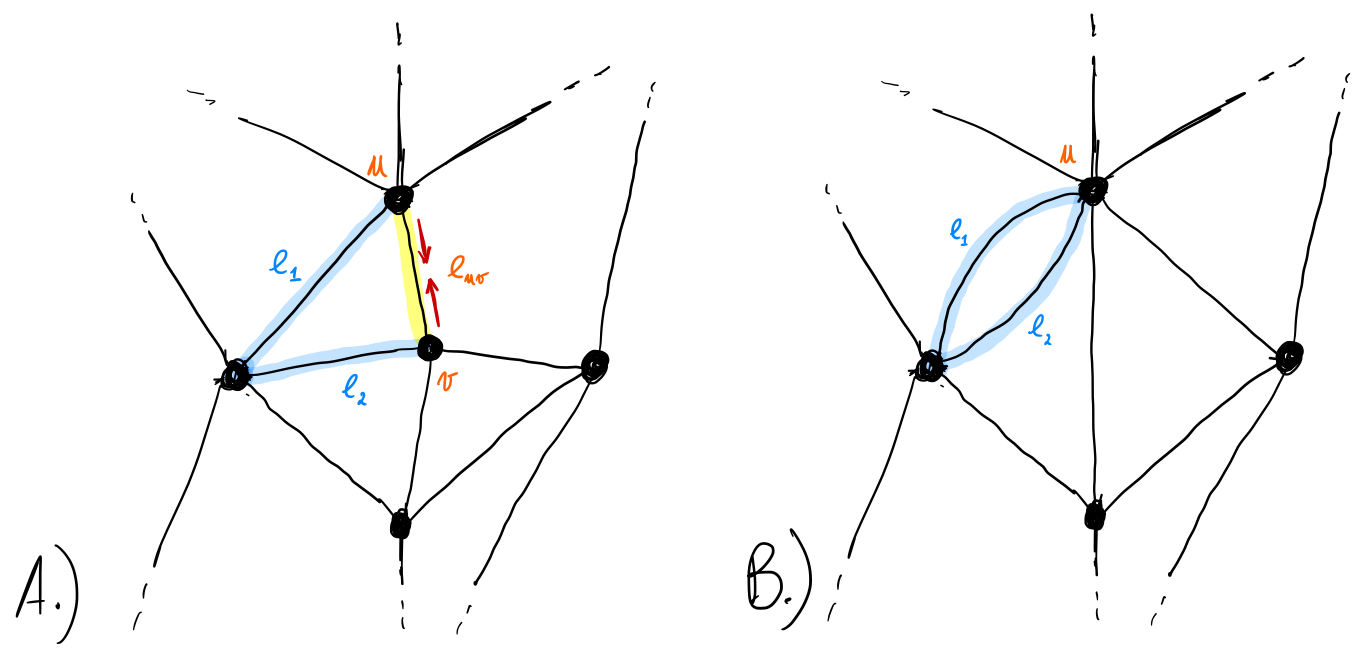
\includegraphics[width=0.50\textwidth,trim=0.in 0.in 0.in 0.in,clip]{./figs/edge_contraction.jpeg}
\caption{\small 
Example of edge contraction: the edge $e_{uv}$ is selected from priority queue; after nodes $u$ and $v$ are merged and $e_{uv}$ is deleted, there are two double edges $e_1$ and $e_2$ left in the graph. 
\label{fig:example_non_unique_weights_1}}
\end{figure}

\begin{figure}
\centering
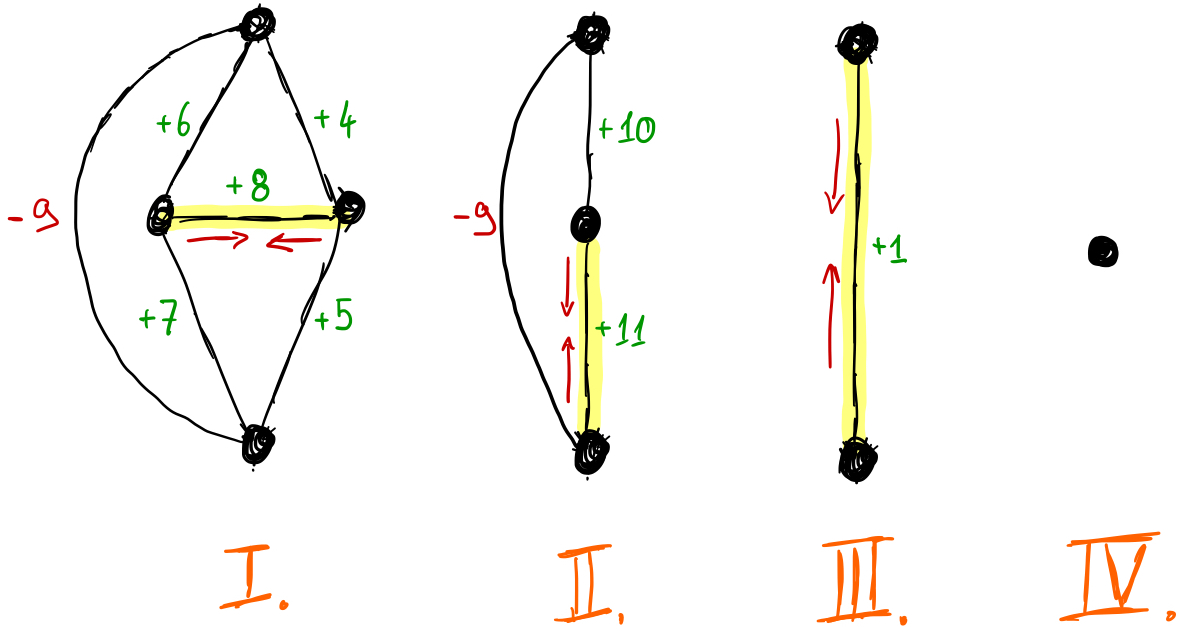
\includegraphics[width=0.45\textwidth,trim=0.in 0.in 0.in 0.in,clip]{./figs/aggl_clust.jpeg}
\caption{\small 
Example of agglomerative clustering on signed graph with sum update rule and... The final clustering is given by one single cluster
\label{fig:example_non_unique_weights_1}}
\end{figure}


\begin{table*}[t]
    \centering
    \begin{subtable}[t!]{0.98\textwidth}\centering
        \begin{tabular}{c | c | c}
            \toprule\toprule
            \makecell{Linkage Criteria\\ (double edges with costs $w_1$ and $w_2$)}                   & \makecell{Algorithm name \\\textbf{without} Must-Not-Link edges}  & \makecell{Algorithm name \\ \textbf{with} Must-Not-Link edges}  \\        
            \midrule\midrule

            Sum: $w_{\mathrm{new}} = w_1+w_2 $                                 & \thead{Greedy Additive \\ Edge Contraction \cite{levinkov2017comparative}} & \thead{Greedy Fixation \cite{levinkov2017comparative}} \\ \midrule
            
            \makecell{$w_{\mathrm{new}}=w_{\tilde{e}}$,$\,
            \,$ where $\tilde{e}=\mathrm{arg}\max_{e\in \{e_{1},e_{2}\}} \left|w_e\right|$  }  & \thead{Mutex Watershed \cite{wolf2018mutex}} & \thead{Mutex Watershed \cite{wolf2018mutex}} \\ \midrule

            Arithmetic mean: $w_{\mathrm{new}} = (w_1+w_2) / 2 $                                 & \thead{Hierarchical Clustering \\ with Average Linkage (UPGMA)} & \thead{\textbf{NEW}}\\ \midrule

            Maximum: $w_{\mathrm{new}} = \max \{ w_1, w_2 \}  $                                 & \thead{Hierarchical Clustering \\ with Single Linkage} & \thead{\textbf{NEW}}\\ \midrule

            Minimum: $w_{\mathrm{new}} = \min \{ w_1, w_2 \}  $                                 & \thead{Hierarchical Clustering \\ with Complete Linkage} & \thead{\textbf{NEW}}



            
        \end{tabular}
        % \caption{Linkage criteria}
    \end{subtable} 
    \caption{Algorithms and linkage criteria}
        \label{tab:linkage-criteria}
\end{table*}


\begin{algorithm}
  \caption{Agglomerative Clustering}
   \hspace*{\algorithmicindent} \textbf{Inputs:} graph $\mathcal{G}(V,E,W)$; boolean {\color{blue}\emph{addMustNotLink}}  \\
  \hspace*{\algorithmicindent} \textbf{Outputs:} Final clustering and contracted graph $\mathcal{G}'$\\
  \hspace*{\algorithmicindent} 
  \begin{algorithmic}[1]


    % \Procedure{SignedGraphEdgeContr}{{\color{blue}bool \emph{addConstraints}}}
      % \State $\mathcal{G}'\gets \mathcal{G}(V,E^+ \cup E^-)$ \Comment{Initialize the contracted graph}
      \State Initialize contracted graph $\mathcal{G}'(V',E')$ from $\mathcal{G}$
      \State Initialize \texttt{canBeMerged}$(e) \gets$ \texttt{True} $\quad \forall e\in E$
      \State Sort edges in priority queue (PQ) in desc. order of $|w_e|$ 
      \State
      \While{PQ is \textbf{not} empty}
        \State Pop edge $e_{uv}\in E'$ with highest abs. priority $|\tilde{w}|$
        \State
        \If{({\color{ForestGreen}\textbf{$\tilde{w} > 0$}}) \textbf{and} \texttt{canBeMerged}$(e_{uv})$}
          
          % \State PQ, $\,E_\dagger,\,\, E' \gets$ \textsc{deleteDoubleEdges}($u,v$)
          
        %   \State Update costs of double edges;
        %   \State Propagate constrained flags of double edges;
          \State Merge nodes $u,v$ and delete $e_{uv}$ from $\mathcal{G}'$
          \State  Replace double edges in $\mathcal{G}'$ with single edges
          \Statex \hspace{\algorithmicindent}\hspace{\algorithmicindent}\hspace{\algorithmicindent} and update priorities
        \EndIf
        % \State
        \If{({\color{red}\textbf{$\tilde{w} \leq 0$}}) \textbf{and} {\color{blue}\emph{addMustNotLink}}}
          % \State Flag $e_{uv}$ as MustNotLink
          \State \texttt{canBeMerged}$(e_{uv}) \gets$ \texttt{False}
        \EndIf
      \EndWhile


      % \For{$e  \in E$ in descending order of absolute costs $|W(e)|$}
      %   \If{({\color{ForestGreen}\textbf{$W(e) > 0$}}) \textbf{AND} (edge is not constrained)}
      %     \State Contract edge $e$ in the graph $\mathcal{G}'$;
      %     \State Update costs of double edges;
      %     \State Propagate constrained flags of double edges;
      %     % \For{every new double edge}
      %     %   \State Delete double edges
      %     %   \State Insert new one with updated cost
      %     % \EndFor
      %   \EndIf
      %   \If{({\color{red}\textbf{$W(e) \leq 0$}}) \textbf{AND} ({\color{blue}\emph{addConstraints}})}
      %     \State Flag edge $e$ as constrained
      %   \EndIf
      % \EndFor
      \State
      \State
      \Return $\mathcal{G}'$
      % \State


    % \EndProcedure

  \end{algorithmic}
\end{algorithm}


\begin{figure}
\centering
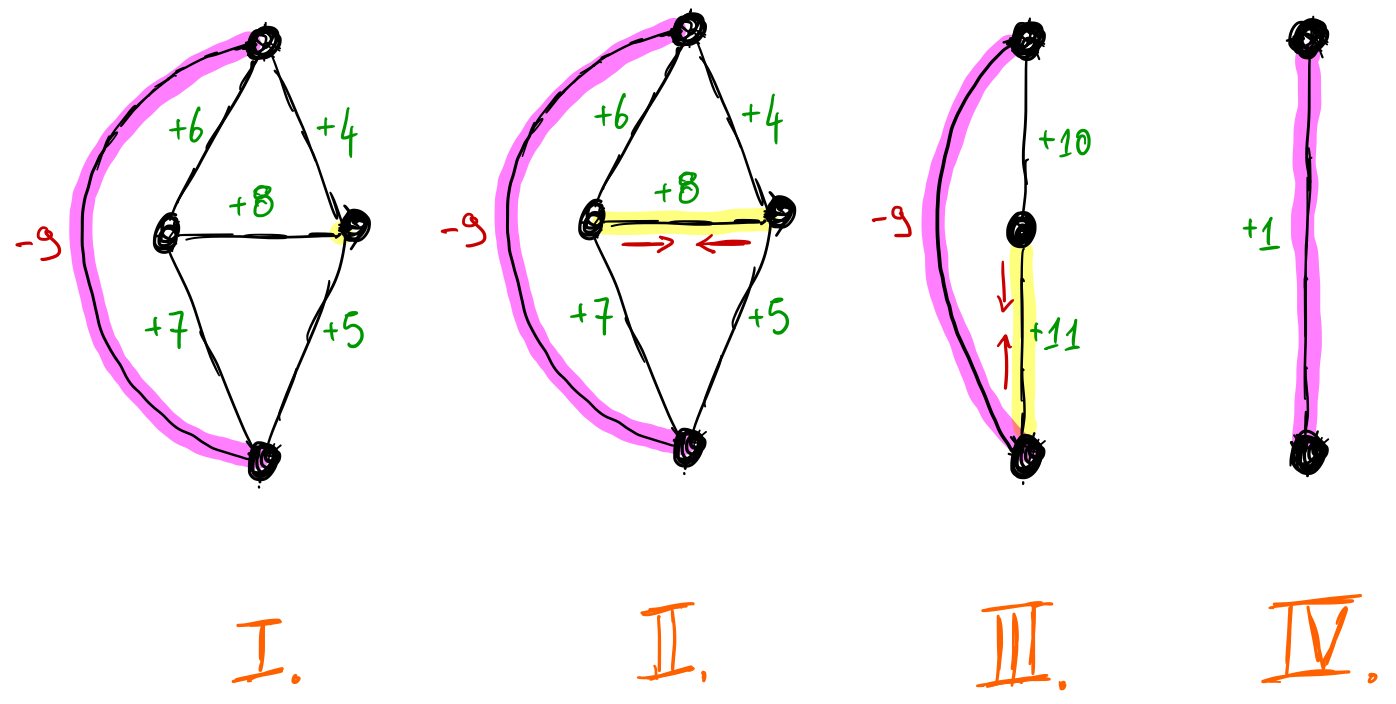
\includegraphics[width=0.50\textwidth,trim=0.in 0.in 0.in 0.in,clip]{./figs/aggl_clust_with_nonlink.jpeg}
\caption{\small 
Example of agglomerative clustering on signed graph with sum update rule and... The final clustering is given by two clusters
\label{fig:example_non_unique_weights_1}}
\end{figure}




% \section{Algorithm}
\section{Agglomerative Clustering}
\begin{itemize}
\item Define graph formalism and clustering $\Pi$
\item Description and pseudo-code
\item Linkage criteria in the table:
\begin{itemize}
\item Mutex Watershed \cite{wolf2018mutex}, [proof of equivalence included in Appendix]
\item Greedy Additive Edge Contraction \cite{levinkov2017comparative}, 
\item Greedy Fixation \cite{levinkov2017comparative}, 
\item Hierarchical Agglomerative Clustering with single, complete, average (UPGMA) linkage criteria
\end{itemize}
\item Easily generalizable for: learned linkage criteria \cite{nunez2013machine}, something depending on node size \cite{felzenszwalb2004efficient}, quantiles, weighted average (WPGMA) and weighted sum

\item Comment about must-not-link relations: they give high priority to the most confident repulsive edges 
\item I don't think I need to mention the merge tree (although it could be easily deduced from the code, as a sequence of clustering)
\item comment about complexity (depends on the linkage criteria) and how dense is the graph (check PQ update)
\end{itemize}


\section{Experiments}
\begin{itemize}
\item define pixel grid graph and long range connections
\item probability of long-range connections
\end{itemize}


% \begin{tabularx}{\columnwidth}{ X | c | c }
%   \toprule
%   \toprule
% Linkage Criteria                   & w/o MNLE & with MNLE \\        
%             \midrule\midrule
%   $w(e_{3})=w(e_{1})+w(e_{2})$  \xdef\tempwidth{\the\linewidth} & top\\\hline
%   \multicolumn{1}{|m{\tempwidth}|}{\lipsum*[1]} & center\\\hline
%   \multicolumn{1}{|b{\tempwidth}|}{\lipsum*[1]} & bottom\\\hline
% \end{tabularx}



\subsection{Qualitative comparison}
\begin{itemize}
\item find good way to represent agglomeration order
\item can we display the must-not-link edges...?
\end{itemize}
\subsection{Noise experiments}

\subsection{Comparison on CREMI and cityscapes}

\section{Conclusions}

\begin{table*}[t]
    \centering
    \begin{subtable}[t!]{0.98\textwidth}\centering
        \begin{tabular}{c | c }
            \toprule\toprule
            \makecell{Algorithm name} & \makecell{Algorithm description and \\linkage criteria}    \\
            \midrule\midrule

            Weighted Arithmetic Mean (WPGMA) & \thead{Assign a weighting $\alpha_e \in \mathbb{R}^+$, $\forall e \in E$ \\ \\ Linkage criteria: $w_{\mathrm{new}} = \frac{\alpha_1 w_1 +\alpha_2 w_2}{\alpha_1 + \alpha_2} $}  \\ \midrule
            
            \makecell{Felzenszwalb Efficient \\Graph-based Image Segmentation \cite{felzenszwalb2004efficient}}  & \thead{Initially all edges have positive weights }  \\ \midrule

            \makecell{Quantile Agglomeration Clustering (...?)}  & \thead{...}  \\ \midrule

            \makecell{Graph-based active learning \\of agglomeration (GALA) \cite{nunez2013machine}}  & \thead{Assign set of edge features $\phi^{\mathrm{I}}_e$ and \\node features $\phi^{\mathrm{II}}_u$, $\forall u \in V$, $\forall e \in E$. \\ \\ A classifier $f$ with parameters $\theta$ predicts and updates\\ the cost of an edge: $w_e = f(\phi^{\mathrm{I}}_e, \phi^{\mathrm{II}}_u, \phi^{\mathrm{II}}_v; \theta)$, $\forall e_{uv} \in E$} \\ \midrule

            % \makecell{$w_{\mathrm{new}}=w_{\tilde{e}}$,$\,
            % \,$ where $\tilde{e}=\mathrm{arg}\max_{e\in \{e_{1},e_{2}\}} \left|w_e\right|$  }  & \thead{Mutex Watershed \cite{wolf2018mutex}} & \thead{Mutex Watershed \cite{wolf2018mutex}} \\ \midrule

            % Arithmetic mean: $w_{\mathrm{new}} = (w_1+w_2) / 2 $                                 & \thead{Hierarchical Clustering \\ with Average Linkage (UPGMA)} & \thead{\textbf{NEW}}\\ \midrule

            % Maximum: $w_{\mathrm{new}} = \max \{ w_1, w_2 \}  $                                 & \thead{Hierarchical Clustering \\ with Single Linkage} & \thead{\textbf{NEW}}\\ \midrule

            % Minimum: $w_{\mathrm{new}} = \min \{ w_1, w_2 \}  $                                 & \thead{Hierarchical Clustering \\ with Complete Linkage} & \thead{\textbf{NEW}}



            
        \end{tabular}
        % \caption{Linkage criteria}
        \label{tab:linkage-criteria}
    \end{subtable} 
    \caption{Linkage criteria 2}
\end{table*}

{\small
\bibliographystyle{ieee}
\bibliography{agglo_clust}
}

\section{Supplementary Material}
\begin{itemize}
\item Equivalence Mutex Watershed and Greedy Edge Contraction
\end{itemize}

\begin{algorithm}
  \caption{Graph Agglomerative Clustering}
\setlength{\parindent}{\algorithmicindent} \textbf{Inputs:}
     \begin{itemize}[leftmargin=1.3cm,topsep=0.1pt,itemsep=-1.ex]
    %  \setlength\itemsep{0.em}
   \item $\mathcal{G}(V,E)$ with $|V|=N$, $|E|=M$
   \item signed edge weights $w:\,E\rightarrow\mathbb{R}$
   \item {\color{blue}addMustNotLink} $\in \{ True, False\}$
   \end{itemize}
   \vspace{0.4em}
   
\setlength{\parindent}{\algorithmicindent} \textbf{Output:} Final clustering $\Pi$

%   \hspace*{\algorithmicindent} \textbf{Inputs:} $\mathcal{G}(V,E)$ with signed costs $w:\,E\rightarrow\mathbb{R}$. \\
%   Prova \\
%   \hspace*{\algorithmicindent} \textbf{Outputs:} Final clustering $\Pi$\\

  \hspace*{\algorithmicindent} 
  \begin{algorithmic}[1]


    % \Procedure{GraphEdgeContr}{{\color{blue}bool \emph{addConstraints}}}
      % \State $\mathcal{G}'\gets \mathcal{G}(V,E^+ \cup E^-)$ \Comment{Initialize the contracted graph}
      \State $\mathcal{G}'(V', E') \gets \mathcal{G}(V, E)$  \Comment{Contracted graph}
    %   \State PQ $\gets$ Sort $e\in E$ in descending order of $|w_e|$
        \State PQ.push$(|w_e|, w_e, e) \quad \forall e \in E $  \Comment{Sort edges by $|w_e|$}
      
      \State $\Pi \gets \{ \{v_1\}, ..., \{v_N\} \}$ \Comment{Initial clustering}
      \State $E_\dagger \gets \{\}$ \Comment{Set of must-not-link edges}
    %   \State PQ.push$(e,  ) \quad \forall e \in E $  
    \State
      \While{PQ is \textbf{not} empty}
        \State $|\tilde{w}|, \tilde{w}, e_{uv} \gets $ PQ.popHighest()
        \If{ $e_{uv} \notin E' $} 
            \State \textbf{continue}
        \EndIf
        \If{({\color{ForestGreen}\textbf{$\tilde{w} > 0$}}) \textbf{and} ($e_{uv} \notin E_\dagger$)}
        %   \State $u,v \gets u,v \in V' : $
        %   \State $S_u \gets S \in \Pi$ : $ u \in S$
        %   \State $S_v \gets S \in \Pi$ : $ v \in S$
          \State PQ, $\,E_\dagger,\,\, E' \gets$ \textsc{deleteDoubleEdges}($u,v$)
        %   \State mergeDoubleEdges($u,v$) \Comment{Update PQ, $E_\dagger, \mathcal{G}'$}
          
        %   \State Update costs of double edges;
        %   \State Propagate constrained flags of double edges;
          \State $V' \gets V' \setminus \{ v\}$, $\quad E' \gets E' \setminus \{ e_{uv}\}$
        %   \State $ S_u \gets S_u \cup S_v$
          \State $\Pi \gets \Pi \cup \{ S_u^\Pi \cup S_v^\Pi \} \setminus \{ S_u^\Pi, S_v^\Pi \}$
          % \For{every new double edge}
          %   \State Delete double edges
          %   \State Insert new one with updated cost
          % \EndFor
        \EndIf
        \If{({\color{red}\textbf{$\tilde{w} \leq 0$}}) \textbf{and} {\color{blue}addMustNotLink}}
          \State $ E_\dagger \gets E_\dagger \cup \{e_{uv} \} $
        \EndIf
      \EndWhile
      \State
    %   \State
      \Return $\Pi$
      % \State
    % \EndProcedure

  \end{algorithmic}
  \hspace*{2cm} 
    \begin{algorithmic}[1]

    \Function{DeleteDoubleEdges}{$u,v$}
      % \State $\mathcal{G}'\gets \mathcal{G}(V,E^+ \cup E^-)$ \Comment{Initialize the contracted graph}
      \State $\mathcal{N}_u = \{ t \in V' | e_{ut}\in E'  \}$
      \State $\mathcal{N}_v = \{ t \in V' | e_{vt}\in E'  \}$
      \For{$t \in \mathcal{N}_u  \cap \mathcal{N}_v$ }
        \State $|\tilde{w}_1|, \tilde{w}_1, e_1 \gets $ PQ.pop($e_{ut}$)
        \State $|\tilde{w}_2|, \tilde{w}_2, e_2 \gets $ PQ.pop($e_{vt}$)
        % \State $e_1, e_2 \gets e_{ut}, e_{vt}$
        \State $E' \gets E' \setminus \{ e_2\}$ %\Comment{Delete double edge}
        \If{$e_2 \in E_\dagger $} \Comment{Propagate must-not-link}
            \State $ E_\dagger \gets E_\dagger \cup \{e_1 \} $
        \EndIf
        % \State $\tilde{w}_1, \tilde{w}_2 \gets $ PQ.pop($e_1$), PQ.pop($e_2$)
        \State $\tilde{w}_{\mathrm{new}} \gets$ \textsc{linkageCriteria}$(\tilde{w}_1, \tilde{w}_2)$
        \State PQ.push($|\tilde{w}_{\mathrm{new}}|$, $\tilde{w}_{\mathrm{new}}$,  $e_1$)
        
        
      \EndFor
      
      \State
    %   \State
      \Return PQ, $E_\dagger, E'$
    %   % \State


    \EndFunction

  \end{algorithmic}
  
\end{algorithm}


\end{document}
